% Chapter Template

\chapter{Método} % Main chapter title

\label{Cap_Exp} % Change X to a consecutive number; for referencing this chapter elsewhere, use \ref{ChapterX}

%----------------------------------------------------------------------------------------
%	SECTION 1
%----------------------------------------------------------------------------------------
\section{Planteamiento general: Poniendo a prueba la existencia del Efecto Espejo en una tarea Perceptual}

%Se propone buscar evidencia del Efecto Espejo en una tarea fuera de Memoria de reconocimiento
El interés principal de la investigación aquí reportada fue buscar los patrones de respuesta reportados en estudios de Memoria de Reconocimiento, identificados como Efecto Espejo, en una tarea de detección ajena a dicha área de estudio.

%Se propone una tarea perceptual ya que carece de una fase de preparacion
En la literatura de Memoria de Reconocimiento existe una tendencia a explicar las diferencias en la ejecución de los participantes entre los tipos de estímulos evaluado apelando a posibles discrepancias en el procesamiento superior de los mismos (por ejemplo, la atención, la recolección de rasgos para su futuro reconocimiento, etc.). Es por eso que en la presente investigación se decidió trabajar con una tarea de detección perceptual, donde las condiciones de discriminabilidad se construyen con base en lo que se ha reportado en la literatura respecto del funcionamiento de nuestros sistemas perceptuales (en específico, en relación a la visión).

%Encontrar evidencia del Efecto Espejo en esta tarea, podría estar sugiriendo que el Efecto Espejo es resultado del uso de SDT para comparar entre dos condiciones de discriminabilidad y no necesariamente del fenómeno de Memoria per se.

El interés principal de la investigación realizada fue evaluar la posibilidad de que el Efecto Espejo, (los patrones de respuesta reportados en estudios de memoria de reconocimiento identificados como tal), sea producto de la aplicación de la TDS  en el análisis y comparación de la ejecución de los participantes entre dos clases de estímulos que tienen diferente nivel de dificultad (i.e. dos niveles de d') y no de una discrepancia a nivel de cómo se procesan los diferentes tipos de estímulo en su primera presentación. Para ello se diseñó una tarea de detección meramente perceptual, donde los tipos de estímulo (los niveles de dificultad) fueron construidos con base en lo reportado por la literatura en ilusiones ópticas.\\ 

%Se trabaja con ilusiones opticas, dado que la literatura en ellas permite anticiparnos a la d' y proponer dos niveles de dificultad.


\subsection{Objetivo}

%Buscar evidencia del efecto espejo en una tarea de detección que no implique el reconocimiento de estimulos ya conocidos.
Determinar si los patrones de respuesta identificados como parte del Efecto Espejo en Memoria de Reconocimiento aparecen también en tareas de detección perceptual con dos niveles de dificultad. Una tarea de este tipo carece de una etapa previa a la experimentación donde los participantes tengan la oportunidad de manipular y procesar distintamente los estímulos que forman parte de la tarea de detección según su dificultad.\\

\section{Construcción de los Experimentos}

%La tarea de detección princiál consiste en comparar el tamaño de dos círculos en pantalla, donde uno de ellos o ambos podía estar construido como una Figura de Ebbinghaus (dependiendo del Experimento)
Se diseñó una tarea de detección perceptual donde los participantes tenían que identificar como 'señal' los ensayos donde dos círculos particulares mostrados en pantalla tuvieran el mismo diámetro. Se construyeron dos variaciones de esta misma tarea: En el primer caso, solo uno de los círculos a comparar fueron consruidos como parte de una figura de Ebbinghaus (Experimento 1); en el segundo, ambos círculos estaban compuestos como parte de una figura de Ebbinghaus diferente (Experimento 2).\\ 

%Descripcion de la Ilusión de Ebbinghaus, la composición de la figura y cómo se explica.
La figura de Ebbinghaus (a.k.a. Círculos de Titchner) suele identificarse como una ilusión óptica que resulta en un fallo en la estimación del tamaño de un círculo cuando este aparece rodeado por un halo de círculos de tamaño uniforme, mayor o menor que el círculo central (Ver Figura~\ref{fig:Ebbinghaus}). La ilusión suele explicarse como producto de la interferencia ocasionada por la estructura de la figura en el sistema cognoscitivo-perceptual que computa el tamaño de los objetos en relación al contraste que tienen con otros elementos en su entorno ($REFERENCIA$). La ilusión de Ebbinghaus puede adoptar dos posibles direcciones: la subestimación y la sobrestimación. La primera se presenta cuando el halo de círculos externos que rodean al círculo central es de mayor tamaño, induciendo la subestimación del tamaño de este último. La segunda, implica el caso contrario donde los círculos externos son más pequeños que el círculo central y llevan a percibir a este último como más grande de lo que en realidad es.\\

\begin{figure}[th]
\centering

\includegraphics[width=0.55\textwidth]{Figures/Ebbinghaus} 
\decoRule
\caption[Ilusión de Ebbinghaus: Ejemplos]{Ilustración de la Ilusión de Ebbinghaus. Los círculos centrales de las dos figuras mostradas tienen el mismo diámetro y sin embargo, el círculo central de la figura izquierda tiende percibirse como más pequeño por el efecto de subestimación elicitado por los círculos circundantes. A su vez, el círculo central derecho suele ser percibido como más grande de lo que de hecho es, por el efecto de sobrestimación producido por el contraste que guarda con los círculos externos.}
\label{fig:Ebbinghaus}
\end{figure}

%Factores o variables que han demostrado influir en la intensidad de la ilusión.
La intensidad de la ilusión provicada por las figuras de Ebbinghaus (i.e. qué tanto se aleja el tamaño estimado del tamaño real del círculo central) suele definirse como una función de las siguientes tres variables: 

\begin{itemize}
\item El tamaño de los círculos externos.
\item La distancia entre el círculo central y el halo de círculos externos.
\item El número de círculos externos.
\end{itemize}

%Descripción del procedimiento empleado por Massaro y Anderson para probar la influencia del numero de circulos externos y el tamaño de los mismos en la Ilusión de Ebbinghaus.
La Figura~\ref{fig:Ebb_Var} presenta los resultados obtenidos por \parencite{Massaro1971} en un experimento que permitió evaluar y valorar el efecto de las variables antes mencionadas en la intensidad de la ilusión de Ebbinghaus. En dicho experimento se construyeron 30 figuras de Ebbinghaus con un diseño factorial de 2x3x5: dos tamaños del círculo central (13 y 17 mm), tres niveles de 'número de círculos externos' (dos, cuatro y seis) y cinco tamaños diferentes de círculos externos (-8, -4, 0, 4 y 8 mm de diferencia respecto del diámetro del círculo central); la distancia entre el círculo central y los círculos externos se mantuvo constante entre las figuras. La tarea de los participantes consistió en elegir un círculo dentro de un set de 27 círculos diferentes cuyos diámetros variaban en un rango de 8.5 a 21.5 mm en intervalos de 0.5 mm, que tuviera el diámetro más cercano al del círculo central de la figura de Ebbinghaus presentada en cada ensayo. En la gráfica se muestra el diámetro promedio elegido por los participantes como más cercano al de los círculos centrales de las figuras de Ebbinghaus construidas (se promedian los datos obtenidos para los dos tamaños de círculo central usados), a lo largo de los distintos niveles de número de círculos externos (en el eje de las abscisas) y por cada valor asignado al diámetro de los círculos externos (señalados con líneas diferentes). El efecto de las manipulaciones propuestas parece ser claro: 1) Entre más círculos externos se incluyen en la figura de Ebbinghaus, mayor es la intensidad de la ilusión, como señala la tendencia las líneas que indica que la diferencia entre el valor real y la estimación de los participantes es cada vez mayor; 2) Mientras mayor sea la diferencia entre el diámetro del círculo central y el de los círculos externos, la intensidad de la ilusión es mayor, como parece indicar la distancia vertical que separa cada una de las líneas. En la figura se distinguen claramente los efectos de sobreestimación y subestimación.\\

\begin{figure}[th]
\centering
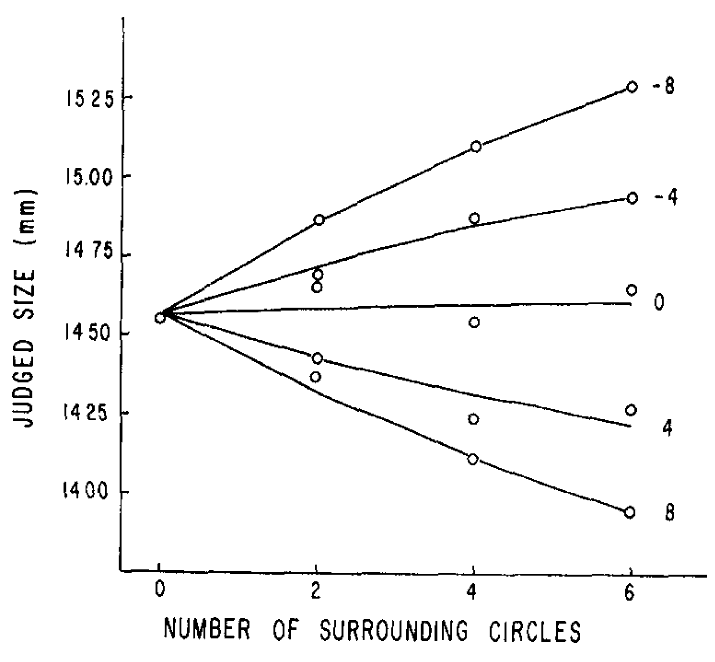
\includegraphics[width=0.55\textwidth]{Figures/Ebb_Variables} 
\decoRule
%\caption[Efecto del Numero y Tamaño de los círculos externos sobre la intensidad de la Ilusión de Ebbinghaus]{Se muestra el efecto que tienen el número de círculos externos incluídos en la ilusión de Ebbinghaus (eje x) sobre los fallos en la estimación del tamaño del círculo central (eje Y); se muestran con líneas diferentes los resultados obtenidos por ilusiones de Ebbinghaus donde los círculos externos diferían en tamaño del círculo central con los valores especificados. La figura fue extraída de la investigación conducida por \parencite{Massaro1971}; Figura 2}
\caption[Efecto del Numero y Tamaño de los círculos externos sobre la intensidad de la Ilusión de Ebbinghaus]{Figura extraída de \parencite{Massaro1971}. Se muestran los resultados obtenidos en un experimento donde se manipuló el número y tamaño de círculos externos para estudiar su efecto sobre la intensidad de la ilusión de Ebbinghaus. La gráfica presenta la estimación promedio de los participantes del diámetro del círculo central de figuras de Ebbinghaus, a través de los distintos niveles de número de círculos externos puestos a prueba (eje de las abscisas), por cada uno de los cinco tamaños de círculos externos utilizados (mostrados en líneas separadas). La tendencia de las líneas a alejarse del estimado promedio en ausencia de círculos externos (sin ilusión inducida), sugiere que a mayor número de círculos externos, mayor es la intensidad de la ilusión. La distancia vertical entre las líneas dibujadas parece indicar que la intensidad de la ilusión aumenta mientras mayor sea la diferencia entre el diámetro del círculo central y el de los círculos externos. Los diámetros estimados se promediaron entre todos los sujetos y entre los dos posibles valores de diámetro del círculo central (13 y 17 mm).}
\label{fig:Ebb_Var}
\end{figure}

%Las condiciones de dificultad estarán determinadas por el número de círculos externos
Con base en los hallazgos reportados por \parencite{Massaro1971} se decidió manipular el número de círculos externos como variable determinante en la construcción de dos niveles de d'. De forma que para la tarea de detección propuesta existiera una condición fácil (con una d' más grande) donde las figuras de Ebbinghaus tuvieron 'pocos' círculos externos (2 o 3 círculos) y una condición difícil (con una d' más pequeña) donde las figuras tuvieron ´'muchos' círculos externos (7 u 8 círculos).\\ 

\subsection{Diseño de los Estímulos}

%En el experimento se trabajó con figuras de Ebbinghaus que promovieran efecto de subestimación Y sobrestimación del tamaño. 
Al diseñar las figuras de Ebbinghaus a utilizar en los experimentos propuestos se incluyeron simultáneamente ilusiones de sobrestimación y subestimación. Para ello se utilizaron dos únicos tamaños para los círculos externos (5 cm y 1 cm), elegidos arbitrariamente de manera que fueran o más grandes que todos posibles círculos centrales (ilusión de subestimación) o más pequeños que la mayoría de los mismos (ilusión de sobrestimación). Es importante hacer notar que el diámetro de los círculos externos en las figuras de Sobrestimación es del mismo tamaño que el círculo central más pequeño contemplado, cancelando el efecto de la ilusión para este caso. Tomando en cuenta que la razón por la que se incluyeron ambos efectos en los experimentos fue para prevenir la habituación y la fatiga de los participantes a la tarea y proveer a la misma cierto dinamismo con una mayor variabilidad en los estímulos presentados, y que el objetivo de la investigación es comparar el desempeño de los participantes entre las condiciones de dificultad propuestas, la inclusión de figuras donde el círculo central y los círculos externos tuvieran el mismo tamaño no se consideró un problema\\

%No se controló la distancia entre el círculo central y los círculos externos.
En ninguno de los experimentos realizados se controló la distancia entre el círculo central y el halo de círculos externos. Al construir las figuras de Ebbinghaus el halo de círculos externos se formó de acuerdo al número de círculos externos, comenzando con las figuras de la condición difícil que contenían entre 7 y 8 círculos externos. Una vez habiendo distribuido los 7 u 8 círculos externos de manera equidistante entre sí en torno al círculo central, se usaron estas mismas figuras como base para la construcción de estímulos de la condición fácil con 2 o 3 círculos externos, borrando los círculos sobrantes y respetando la ubicación de los restantes respecto del círculo central; para las figuras con 2 círculos externos, se procuró que estos estuvieran enfrentados en puntos opuestos del círculo central y para las figuras con tres círculos centrales se procuró que estos estuvieran localizados de manera tal que formasen un ángulo de $CIENTO VEINTE GRADOS$ entre sí. El tamaño impuso una restricción importante en la formación de estos halos de 7 u 8 círculos externos, por lo que su localización permaneció constante a lo largo de los distintos tamaños de círculo central, modificando en consecuencia la distancia entre estos. Es en este sentido que se habla de una falta de control en la distancia entre los círculos centrales y el halo de círculos externos. Sin embargo, apelando nuevamente a que dichas distancias permanecen constantes entre condiciones de dificultad, no se consideró una fuente de ruido importante para analizar lo que se propuso en la tarea: diferencias en el desempeño dependientes del número de círculos externos.\\

A continuación, se desarrolla con detalle la construcción de los estímulos (Señales y ruido) utilizados en cada uno de los dos experimentos realizados. Las especificaciones respecto al procedimiento, las tareas y los controles realizados en los experimentos se explican a profundidad, más adelante.\\

\begin{itemize}
\item Experimento 1 : Circulo de referencia aislado vs Figura de Ebbinghaus.

%Los ensayos de la tarea de detección están compuestos por un círculo aislado constante del lado izquierdo, cuyo tamaño debe ser comparado con el círculo central de una figura de Ebbinghaus en el lado derecho de la pantalla.
En el Experimento 1 sólo se mostraba una figura de Ebbinghaus por ensayo, siempre en la mitad derecha de la pantalla, cuyo círculo central los participantes tenían que comparar con un círculo de referencia de 2 cm de diámetro, con localización fija en la mitad izquierda de la pantalla, para determinar si su tamaño era el mismo (señal) o no (ruido). Los círculos a comparar aparecían a la misma altura de la pantalla. El círculo de referencia y el círculo central de las figuras de Ebbinghaus aparecían 14 cm a la izquierda y 10 cm a la derecha del centro de la pantalla, respetivamente.\\

%Desarrollo del diseño factorial de 5x2x2 utilizado para construir los estímulos del Experimento 1: 5 circulos centrales x 2 tipos de ilusion x 2 niveles de 'numero de circulos externos'
Las figuras de Ebbinghaus utilizadas en el Experimento 1 se diseñaron de acuerdo a un diseño factorial de 5x2x2, (Ver Figura~\ref{fig:Exp_1}). Se utilizaron cinco diferentes tamaños de círculo central, partiendo del tamaño del círculo de referencia (2 cm; la combinación con la señal) y alejándose de este en saltos de 0.5 cm en ambas direcciones (i.e. Círculos más pequeños que la referencia, de 1 y 1.5 cm, y círculos más grandes que la referencia, de 2.5 y 3 cm de diámetro). Por cada uno de estos cinco tamaños de círculo central, se construyeron dos tipos de figuras de Ebbinghaus dependientes del tamaño de los círculos externos: grande (efecto de subestimación) y pequeño (efecto de sobrestimación). Por último, por cada una de estas 10 combinaciones, se hicieron dos figuras diferentes de acuerdo a los niveles de 'número de círculos externos' propuestos por condición (2 y 3 círculos en la condición fácil; 7 y 8 círculos en la condición difícil). Esto nos deja con un subtotal de 20 figuras diferentes por condición y un total de 40 en todo el experimento.\\
 
%Los estímulos con ruido se presentaron 10 veces durante el experimento. Los estímulos con señal se presentaron con 40 repeticiones. La discrepancia en el número de repeticiones entre ambos tipos de estímulo se hizo para igualar la  
El set de figuras de Ebbinghaus construido contiene una mayor cantidad de estímulos con ruido (32 figuras con ruido; 16 por condición) que con señal (8 figuras con la señal; 4 por condición). Para procurar que los participantes se encontraran con la misma cantidad de ensayos con señal que con ensayo con ruido, se incrementó el número de repeticiones con que las figuras con señal aparecieron en el experimento. Cada una de las 32 figuras de Ebbinghaus con ruido se presentó en diez ocasiones diferentes durante el experimento, mientras que las ocho figuras con señal tuvieron 40 repeticiones por cada una. De esta forma, el experimento terminó compuesto por 320 ensayos con ruido y 320 ensayos con señal, 160 ensayos por cada condición de dificultad para ambos tipos de estímulo. La inclusión homogénea de ensayos con ruido y señal se realizó con el fin de que la discrepancia en la aparición de un caso sobre otro no proviera información que sesgara la respuesta de los participantes hacia la emisión de juicios negativos ('No, no son iguales').\\

\begin{figure}[th]
\centering
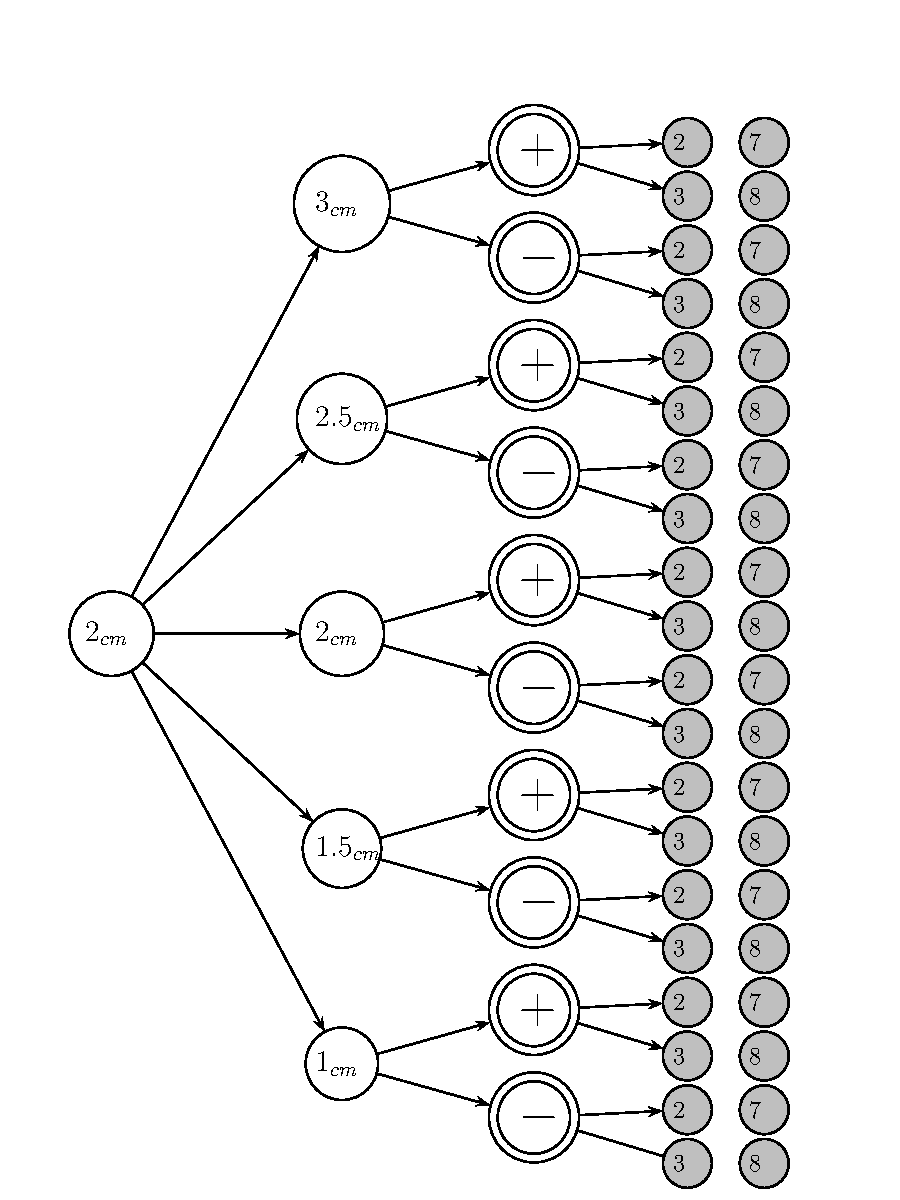
\includegraphics[width=0.99\textwidth]{Figures/Estimulos_Experimento1} 
\decoRule
\caption[Diseño de Estimulos en el Experimento 1]{Diseño factorial (5x2x2) utilizado para construir los estímulos utilizados durante la tarea de detección en el Experimento 1. En cada ensayo los participantes tenían que comparar el tamaño de un círculo de referencia constante con el círculo central de una figura de Ebbinghaus, que podía aparecer en cinco posibles tamaños, con círculos externos que inducen efectos de sobrestimación o subestimación (indicado en el esquema con  y signos positivos y negativos, respectivamente) y con dos niveles de 'número de círculos externo' por condición (2 y 3 círculos externos en la condición fácil o 7 y 8 en la condición difícil). Por cada condición de dificultad, se tienen 16 estímulos con ruido, (10 repeticiones por cada uno, en cinco colores diferentes) y 4 que contienen la señal (repetidos 40 veces cada una, en cinco colores diferentes), dejándonos con 320 ensayos por condición y un total de 640 ensayos en el experimento.}
\label{fig:Exp_1}
\end{figure}

%Las repeticiones de cada figura aparecieron en cinco colores diferentes para prever la fatiga.
Procurando evitar la fatiga en los participantes, cada uno de los estímulos diseñados apareció en cinco colores diferentes (Guinda, Anaranjado, Verde, Azul y Púrpura) en cantidades iguales (Dos estímulos de cada color dentro de las 10 repeticiones de estímulos con ruido y 8 estímulos de cada color dentro de las 40 repeticiones de estímulos con señal). Para todos los casos, el círculo central se mostró en un tono más claro que los círculos externos. Estas diferencias en el tono y color de las figuras han demostrado no tener un efecto en la intensidad de la ilusión $REFERENCIA$ y fueron incluidas con la única intención de tener una mayor variabilidad en los estímulos presentados y que los participantes no se harten ni se aburran de la tarea, ambos estados que podrían mermar la atención con que responden a la misma. 

\item Experimento 2 : Figura de Ebbinghaus (Sobrestimación) vs Figura de Ebbinghaus (Subestimación).

%En la tarea de detección, los participantes tenían que comparar el círculo central de dos figuras de Ebbinghaus que aparecían simultáneamente en la pantalla: una con círculos externos grandes (Efecto de subestimación)  y una con círculos externos pequeños (Efecto de sobrestimación).
En el Experimento 2 los participantes tenían que comparar el tamaño del círculo central de dos figuras de Ebbinghaus que aparecían simultáneamente en pantalla. Al igual que en el Experimento 1, las respuestas se reportaban presionando una de dos posibles teclas para señalar si los círculos a comparar tenían el mismo tamaño (la señal) o no (el ruido). Las parejas construidas contenían ambos tipos de ilusiones: una figura con efecto de subestimación (con círculos externos grandes; 6 cm de diámetro) y una figura con efecto de sobrestimación (con círculos externos pequeños; 1 cm de diámetro). Los círculos centrales aparecían en pantalla a la misma altura, a -15 y 11 cm respecto del centro de la pantalla.\\


%Se formaron cinco parejas con la Señal (cinco pares iguales de tamaño de círculo central) y cinco parejas con el ruido (cuatro cuyos círculos centrales diferían en 0.5 cm y una que difería en 1 cm).
La Figura~\ref{fig:Exp_2} ilustra el diseño de las figuras de Ebbinghaus utilizadas en el Experimento 2. A diferencia del Experimento 1, donde uno de los círculos a comparar permanecía constante, en el Experimento 2 se varió el diámetro de los dos círculos a comparar dentro de un rango de cinco valores, de 1 a 3 cm en saltos de 0.5 cm, construyendo así cinco tipos posibles de Parejas-señal. Por su parte, las Parejas-ruido se formaron arbitrariamente, empatando círculos centrales cuyo diámetro difiriese en 0.5 cm (i.e 1 vs 1.5 cm; 1.5 vs 2 cm; 2 vs 2.5 cm y 2.5 vs 3 cm), con una quinta pareja donde la diferencia se extendía hasta 1 cm, entre los valores menos extremos (1.5 cm vs 2.5 cm). Para cada una de estas 10 parejas, se crearon cuatro nuevas versiones para cada condición, de acuerdo con las posibles combinaciones de los niveles de 'número de círculos centrales' (2 círculos externos a ambos lados, 3 círculos externosa ambos lados, 2 en izquierdo y 3 en derecho y 3 en izquierdo y 2 en derecho, para la condición fácil; 7 círculos externos a ambos lados, 8 círculos externos ambos lados, 7 círculos del lado izquierdo y 8 en el derecho y 8 círculos en el lado izquierdo y 7 en el derecho). En total, el Experimento 2 estuvo compuesto por 80 parejas diferentes de figuras de Ebbinghaus cuyos círculos centrales debían compararse; 40 por condición; 20 por cada tipo de estímulo en cada condición.\\

\begin{figure}[th]
\centering
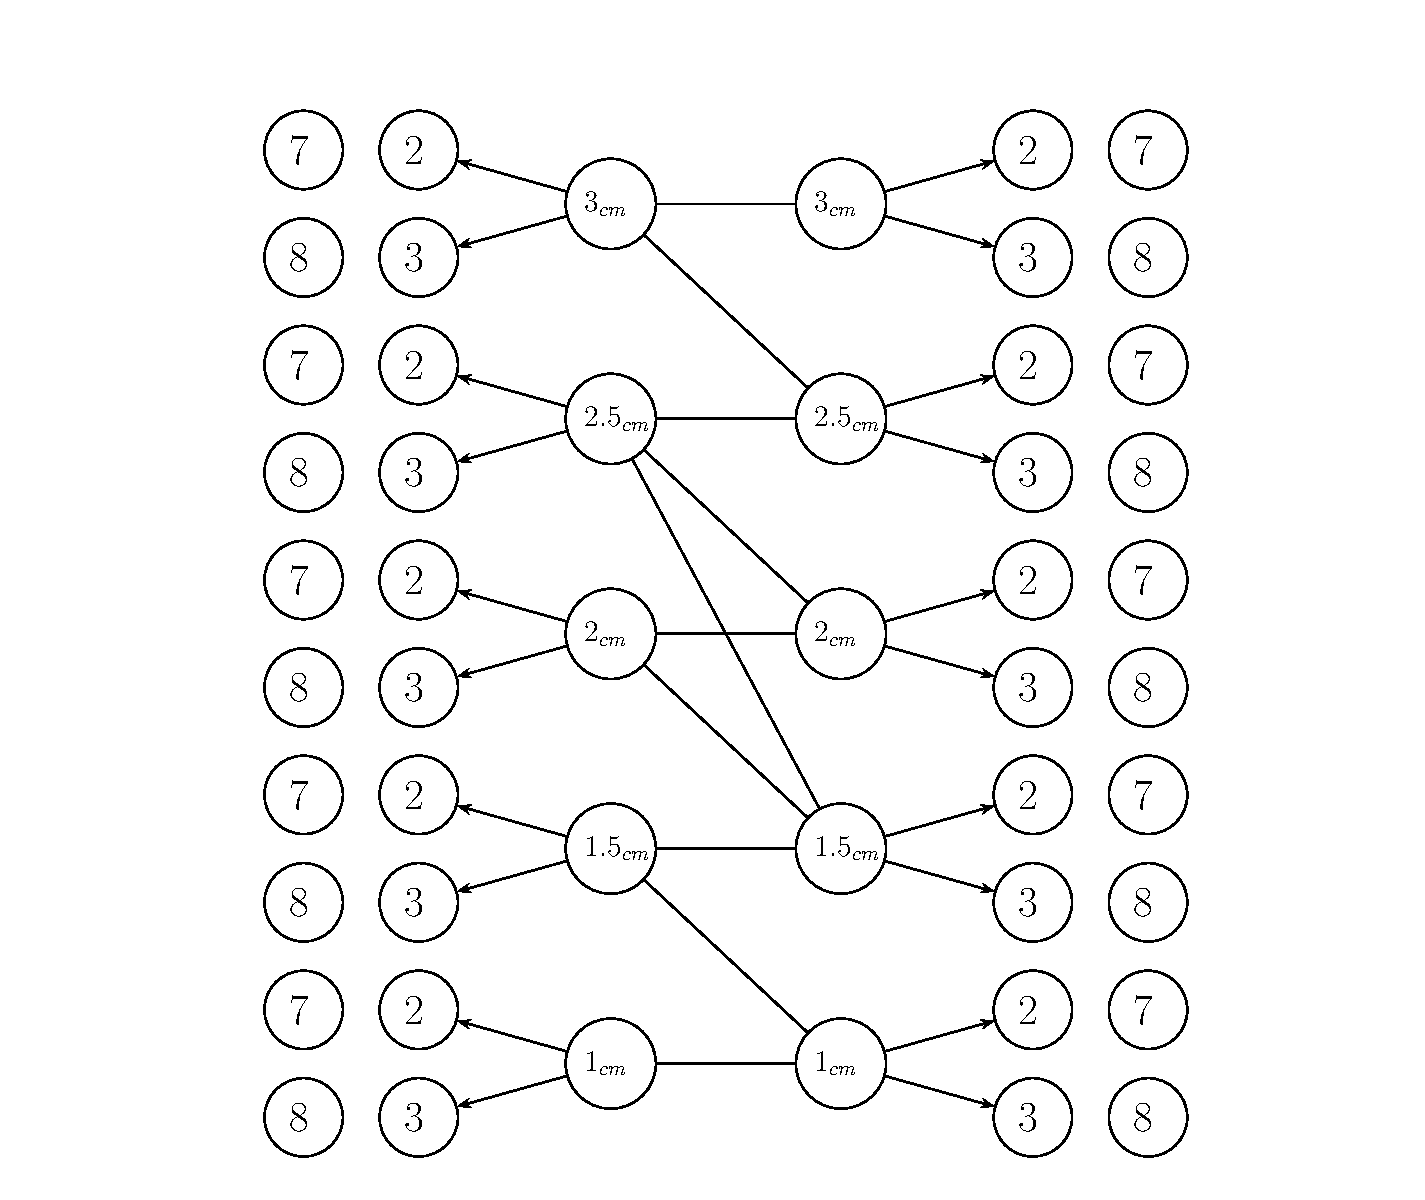
\includegraphics[width=1.2\textwidth]{Figures/Estimulos_Experimento2} 
\decoRule
\caption[Diseño de Estimulos en el Experimento 2]{Diseño de las parejas  de figuras de Ebbinghaus a comparar en el Experimento 2. Se manejaron cinco tamaños distintos de círculo central, que se mostraron en parejas iguales (cinco señales) y cinco parejas desiguales (cuatro cuyos círculos centrales diferían en 0.5 cm y, una con una diferencia de 1 cm). En cada pareja siempre había una figura de Ebbinghaus que inducía la subestimación del tamaño central y una que promovía la subestimación, contrabalanceando el orden en que aparecían en pantalla (relativo a la posición izquierda o derecha). Por cada pareja de círculos centrales, se contemplaron cuatro combinaciones posibles entre los dos niveles de círculos externos contenidos por cada condición (i.e. a vs a, b vs b, a vs b, b vs a; donde a y b son sustituíbles por 2 y 3 círculos externos en la condición fácil o 7 y 8, en la condición difícil.)}
\label{fig:Exp_2}
\end{figure}
\end{itemize}

%Cada pareja diseñada se repitió 8 veces; en 4 colores diferentes y contrabalanceando la ubicación de cada tipo de ilusión. En total, el Experimento 2 estuvo compuesto por 640 ensayos.
Cada una de las 80 parejas diseñadas para el Experimento 2 se presentó 8 veces, en cuatro colores diferentes (púrpura, anaranjado, azul y verde) para prevenir la fatiga de los participantes, contrabalanceando además la ubicación de las ilusiones de sobrestimación y subestimación a la derecha o izquierda de la pantalla. En otras palabras, por cada pareja construida de figuras a comparar se incluyeron ocho ensayos en el experimento: con un par de cada uno de los cuatro colores propuestos, dentro de los cuales se variaba la localización de las ilusiones a la derecha o izquierda, con un caso de cada combinación posible (i.e. Sobrestimación - Subestimación vs Subestimación - Sobrestimación). De tal forma que el Experimento 2 estuvo compuesto por un total de 640 ensayos; 320 por cada condición y 160 por cada tipo de estímulo por condición.\\ 

\subsection{Materiales}

%Programacion de la tarea
La tarea fue programada y ejecutada en PsychoPy v.12, un paquete de libre acceso programado en lenguaje Python que facilita la generación de tareas experimentales en psicología y neurociencias.  

%Detalles sobre la Mac y el espacio utilizado para correr el experimento.
El experimento se corrió en una computadora de escritorio Mac, con una pantalla de $medidas$, en un cubículo interno dentro del laboratorio 25 del Edificio D de la Facultad de Psicología de la UNAM.

\subsection{Participantes}

%Total de participantes y distribucion entre experimentos.
Un total de cuarenta y un estudiantes de la Facultad de Psicología participaron en los experimentos planteados: veinte en el Experimento 1 y veintiuno en el Experimento 2. Los experimentos se llevaron a cabo de manera simultánea. Los participantes fueron asignados a los experimentos alternadamente, procurando terminar con una cantidad similar de participantes en cada uno.\\

%Procedencia y generalidades sobre los participantes.
Todos los participantes fueron estudiantes de los primeros cuatro semestres de la licenciatura en Psicología de la Facultad de Psicología de la Universidad Nacional Autónoma de México, cuyas edades variaban entre los 18 y los 21 años. Su participación fue incentivada con el ofrecimiento de un boleto para la rifa de una tarjeta de regalo con valor de $TRESCIENTOS PESOS$ pesos para la plataforma de su preferencia entre iTunes, Netflix y Amazon. Se realizaron dos rifas independientes, una por cada experimento. Sin embargo, pese a que se informó a los participantes de la existencia de dos experimentos diferentes con su respectiva rifa, nunca se les proporcionó información respecto a cuál habían sido asignados.\\ 

%Consentimiento informado.
Para participar en el experimento se solicitó a cada participante que firmara una carta de consentimiento individual donde se les informaba la duración estimada de la tarea (40 minutos para cualquiera de los experimentos), se confirmaba su participación en una de las rifas y se les advertía que el procedimiento podría resultar fatigoso y que, aunque su participación era voluntaria y podían dimitir en cualquier momento, su permanencia en el mismo hasta el final era crucial para poder utilizar sus datos. De manera adicional, todos los participantes proporcionaron número(s) de teléfono y correo electrónico como medio de contacto.\\

\section{Procedimiento}

%Los experimentos propuestos difieren en el tipo de estímulos a presentar. Sin embargo, la tarea principal y el resto de los detalles del procedimiento permanecen iguales para ambos casos. 
La diferencia primordial entre los Experimentos 1 y 2 tiene que ver con el tipo de estímulos presentados a los participantes: en un caso se compara el círculo central de una figura de Ebbinghaus contra un círculo de referencia fijo (Experimento 1) y en el otro, se muestran simultáneamente dos figuras de Ebbinghaus cuyos círculos centrales deben compararse. La tarea es la misma (comparar el diámetro de dos círculos específicos que se muestran en la pantalla), de la misma forma que el resto del procedimiento a seguir y los detalles con que este fue programado.\\

%La tarea de detección constaba de dos fases: 1) Una tarea de detección binaria (¿Son o no del mismo tamaño?) y 2) Una tarea con escala de confianza (¿Qué tan seguro estás de tu respuesta?)
Los experimentos incorporaron dos procedimientos diferentes para evaluar la tarea de detección propuesta: una pregunta de respuesta binaria 'Sí/No' y una escala de confianza sobre esta primer respuesta.\\

Después de haber firmado la carta de consentimiento informado, se instalaba a los participantes en el espacio asignado para la realización del experimento. En el monitor de la computador designada se mostraba una pantalla inicial que daba la bienvenida a los participantes al Laboratorio 25 de la Facultad de Psicología de la Universidad Nacional Autónoma de México. En cuanto el participante oprimía la barra espaciadora comenzaban a desplegarse las instrucciones para responder al experimento ($REFERENCIA A APENDICES$), que incluían un ejemplo de cómo se verían los estímulos a comparar de acuerdo con el experimento realizado. Las instrucciones finalizaban con una pantalla en blanco con la leyenda 'Presiona la barra espaciadora para comenzar el experimento', que daba oportunidad a los participantes de comenzar el experimento en cuanto estuvieran listos.\\

La estructura de cada ensayo fue la siguiente:\\

\begin{itemize}
\item Fase 1: Tarea de respuesta binaria 'Sí/No'

En esta primera fase, se mostraba a los participantes los círculos a comparar para que indicaran, presionando una de dos posibles teclas, si sus diámetros eran o no del mismo tamaño. Si los círculos eran percibidos como iguales, los participantes debían presionar la tecla 'S'; en caso contrario, 'N'.

En cada ensayo se mostró a los participantes uno de los estímulos a comparar acompañado por un par de leyendas en la parte superior e inferior de la pantalla, respectivamente. Estas leyendas fueron colocadas a manera de recordatorio para los participantes: en la parte superior de la pantalla se les recordaba la pregunta de detección a responder (i.e. ¿Los círculos centrales son del mismo tamaño?) y en la parte inferior, las teclas que debían presionar para emitir su respuesta (i.e. 'S = Sí, N = No'). Como ejemplo de cómo se veían los ensayos experimentales en los Experimentos 1 y 2, ver las Figuras $FIGURAS DE EJEMPLO$, respectivamente.\\

Los estímulos se mostraban en pantalla sólo por 1.5 segundos para preveer la habituación de los participantes a la ilusión, con independencia de si se hubiera emitido una respuesta antes de finalizado el intervalo. Si el participante respondía antes de 1.5 s, los estímulos se quedaban en pantalla hasta terminar dicho periodo, tras el cual se avanzaba inmediatamente a la siguiente fase del ensayo. Si el participante no había registrado su respuesta aún después de la desaparición del estímulo, las leyendas-recordatorios permanecían en pantalla hasta que esta fuese emitida.\\

\item Fase 2: Escala de Confianza

%En una segunda fase, los participantes tuvieron que oprimir una tecla del 1 al 3 para indicar qué tan seguros estaban de la respuesta recién emitida.
Una vez registrada la respuesta de los participantes a la tarea 'Sí/No', comenzaba la Fase 2 del ensayo. En esta ocasión, los participantes tenían que presionar una tecla del 1 al 3 que reflejara qué tan seguros se sentían de la respuesta recién dada en la fase anterior. Para esto, se desplegaba en pantalla una tabla que recordaba a los participantes las opciones de respuesta y su significado (i.e. '1, Poco seguro; 2, Más o menos seguro; 3, Muy seguro') debajo de la pregunta guía '¿Qué tan seguro estás de tu respuesta?'. \\

El puntaje asignado por el participante (1,2,3) para valuar su certidumbre en la respuesta dada en la fase anterior, fue convertido y registrado por el programa como parte de una escala más grande, con valores del 1 al 6, que distingue entre la confianza que se pueda tener en que el estímulo a evaluar contenga sólo ruido ('1 = Muy seguro de que NO es la señal'; '2 =  Más o menos seguro de que NO es la señal'; '3 = Poco seguro de que NO es la señal') y la confianza de que se trate de un estímulo con señal ('4 = Poco seguro de que es la señal'; '5 = Más o menos seguro de que es la señal'; '6 = Muy seguro de que es la señal'). Los valores extremos de esta nueva escala, representan la mayor seguridad en las posibles respuestas a emitir en la fase anterior 'Sí/No', representando con los valores intermedios una mayor incertidumbre entre cuál de estas pudiera ser la más apropiada para responder al ensayo en cuestión. La conversión del número elegido por el participante en el experimento en esta nueva escala se hizo tomando en cuenta la respuesta del participante a la tarea 'Sí/No', de la siguiente manera.\\

\begin{itemize}
\item En los ensayos en que el participante hubiera respondido 'No' a la pregunta '¿Los círculos centrales son del mismo tamaño?', la conversión del puntaje asignado habría sido la siguiente forma:\\
	\begin{itemize}
	\item '1 = Estoy poco seguro de mi respuesta', habria sido convertido en un '3'.\\
	\item '2 = Estoy más o menos seguro de mi respuesta', habría conservado el valor '2'.\\
	\item '3 = Estoy muy seguro de mi respuesta', habría correspondido a un nuevo valor de '1'.\\
	\end{itemize}
\\
\item En los ensayos donde el participante hubiera respondido 'Sí' a la pregunta descrita para la primera fase, la transformación de puntajes asignados habría seguido la siguiente lógica:\\
	\begin{itemize}
	\item '1 = Estoy poco seguro de mi respuesta', se habría movido hacia el '4'.\\
	\item '2 = Estoy más o menos seguro de mi respuesta', habría sido transformado en '5'.\\
	\item '3 = Estoy muy seguro de mi respuesta', habría pasado a '6'.\\
	\end{itemize}
\end{itemize}

Esta nueva escala de 6 elementos que distingue entre la certeza de que se trate de un ensayo con ruido y la seguridad de que se trate de una señal nos permite evaluar la ejecución de los participantes más allá de la definición de un criterio único de elección que determina si responden 'Sí' o 'No' a cada ensayo. Teóricamente, a partir de la valoración hecha por los participantes respecto de qué tan seguros se sienten de identificar cada uno de los estímulos a evaluar como parte de la muestra de señales o ruido, podremos ubicar no uno, sino seis sub-criterios de elección que van a determinar a partir de cuánta evidencia el participante comienza a sentirse más, o menos seguro, de que el ensayo a evaluar contiene sólo ruido o una señal. Para una representación gráfica de cómo funciona y cuál es el propósito de esta segunda fase de los ensayos, ver la figura $ INSERTAR FIGURA $\\

Una vez registrada la segunda respuesta del participante (i.e. el puntaje asignado a la escala de confianza), se daba por terminado el ensayo.\\

\end{itemize}

%Entre cada ensayo, se presentó una pantalla intermedia que solicitaba a los participantes presionar la barra espaciadora para indicar que estaban listos para responder al siguiente ensayo.
Al finalizar cada ensayo se mostraba a los participantes una pantalla 'de pausa' que daba a los participantes la oportunidad de señalar cuando estuvieran listos para atender y responder al siguiente par de estímulos a comparar presionando la barra espaciadora. Estas pantallas entre ensayos fueron incluidas para garantizar que los participantes pudieran atender y evaluar los círculos a comparar durante el periodo de exposición de los mismos.\\

Al terminar los 640 ensayos que conformaron el experimento, a manera de conclusión, se mostró a los participantes una pantalla que contenía la retroalimentación general de su desempeño durante la tarea (i.e. el número de aciertos y errores cometidos a lo largo de todo el procedimiento). En ningún momento se informó a los participantes sobre las variables manipuladas durante el experimento (i.e sobre la existencia de dos clases de estímulos distinguidas por su nivel de dificultad).\\ 

%Se registraron tiempos de respuesta por cada respuesta registrada (Respuesta en la tarea Sí/No; Respuesta en la escala de confianza) y  la duración del experimento completo.
Se registraron los tiempos de respuesta de los participantes a las diferentes fases del experimento. Por cada ensayo, se registraron el tiempo de respuesta de los participantes a la tarea binaria tras la aparición de los estímulos a comparar y el tiempo de respuesta a la escala de confianza. También se registró el tiempo total que tomó a los participantes finalizar el experimento, desde que presionaran la barra espaciadora para comenzar las instrucciones hasta que hubieran respondido al último de los 640 ensayos y hubieran recibido la retroalimentación global de su ejecución.\\

%Controles
Todos los participantes realizaron el experimento sentados en una silla fija, cuyo centro se encontraba a un metro de la pantalla principal. Se solicitó a los participantes que no llevaran el celular consigo al espacio de experimentación, para preveer posibles distracciones. \\

\subsection{Registro de respuestas}

El experimento fue programado de manera tal que los datos obtenidos sobre la ejecución de cada participante se vaciaran en un documento en formato csv, con el título del mismo indicando el número e iniciales del participante, el día en que se este hubiera participado en el experimento y el experimento en que participó.\\

\begin{figure}[th]
\centering
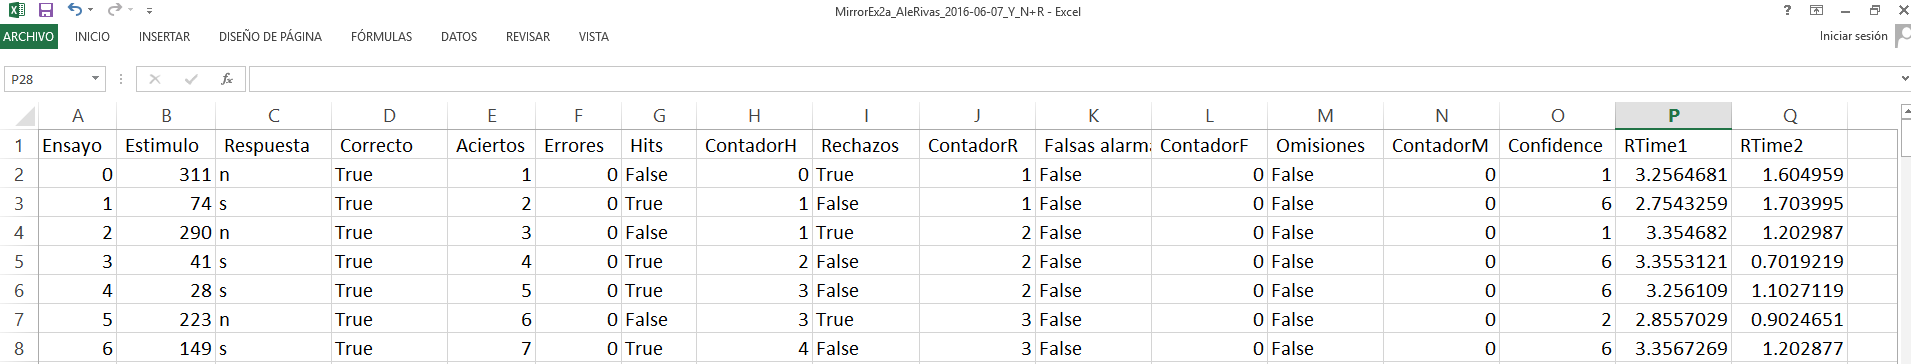
\includegraphics[width=0.95\textwidth]{Figures/csv} 
\decoRule
\caption[Csv muestra]{Captura de pantalla de uno de los archivos csv generados tras la aplicación del experimento. Se ilustra el registro y clasificación de las respuestas emitidas por los participantes en cada ensayo, en función de su correspondencia con el estímulo aleatoriamente mostrado. Se muestran únicamente los primeros seis ensayos del Experimento 2, realizado el 7 de junio del 2016.}
\label{fig:csv}
\end{figure}
\end{itemize}

La figura~\ref{fig:csv} muestra como ejemplo los primeros seis ensayos registrados en uno de los csv's obtenido tras la realización de nuestro experimento. El csv se fue escribiendo por nuestro programa conforme van avanzando los ensayos, indicándonos cuál de los estímulos diseñados (Estímulo) fue seleccionado aleatoriamente para aparecer en cada ocasión (Ensayo); para señalar el estímulo presentado en cada ensayo se utilizaron números arbitrariamente asignados a cada una de las combinaciones generadas para la elaboración de las figuras de Ebbinghaus (ver las $FIGURAS DE DISEÑO DE ESTIMULOS$). La respuesta del participante se registra (Respuesta) y se clasifica como Correcta o no (se escribe 'True' o 'False' en la columna 'Correcto') de acuerdo a su correspondencia con el estímulo que apareció en pantalla. A continuación, se presentan dos columnas que van registrando la frecuencia acumulada con que el participante acierta y se equivoca a lo largo del experimento (Aciertos y Errores, respectivamente). Además de indicar si se trata de una respuesta acertada, o no, el programa identifica la respuesta emitida por el participante en función a qué tipo de acierto puede ser (Hit o Rechazo) y a qué tipo de error (Falsa alarma u Omision), llevando un contador para cada uno de estos casos que muestra la frecuencia acumulada con que el participante emite una respuesta de cada tipo (ContadorH, para los Hits; ContadorR, para los Rechazos correctos; ContadorF, para las Falsas Alarmas; ContadorM, para las omisiones). En cuanto a la segunda fase de cada ensayo, se registra el puntaje obtenido al aplicar la conversión previamente detallada al número elegido por el participante a la escala de confianza en su respuesta presentada (Confidence). Por último se muestran los Tiempos de Respuesta registrados por cada ensayo: RTime1, corresponde al tiempo de respuesta transcurrido a partir de la aparición del estímulo en pantalla; RTime1b muestra el tiempo transcurrido desde la desaparición del estímulo en pantalla y la emisión de la respuesta del participante; RTime2 presenta el tiempo de respuesta a la segunda fase de cada ensayo.\\ 

